%  for submission AI in Ed Journal.
%  http://iaied.org/journal/authors/
%% bare_conf.tex
%% V1.3
%% 2007/01/11
%% by Michael Shell
%% See:
%% http://www.michaelshell.org/
%% for current contact information.
%%
%% This is a skeleton file demonstrating the use of IEEEtran.cls
%% (requires IEEEtran.cls version 1.7 or later) with an IEEE conference paper.
%%
%% Support sites:
%% http://www.michaelshell.org/tex/ieeetran/
%% http://www.ctan.org/tex-archive/macros/latex/contrib/IEEEtran/
%% and
%% http://www.ieee.org/

%%*************************************************************************
%% Legal Notice:
%% This code is offered as-is without any warranty either expressed or
%% implied; without even the implied warranty of MERCHANTABILITY or
%% FITNESS FOR A PARTICULAR PURPOSE!
%% User assumes all risk.
%% In no event shall IEEE or any contributor to this code be liable for
%% any damages or losses, including, but not limited to, incidental,
%% consequential, or any other damages, resulting from the use or misuse
%% of any information contained here.
%%
%% All comments are the opinions of their respective authors and are not
%% necessarily endorsed by the IEEE.
%%
%% This work is distributed under the LaTeX Project Public License (LPPL)
%% ( http://www.latex-project.org/ ) version 1.3, and may be freely used,
%% distributed and modified. A copy of the LPPL, version 1.3, is included
%% in the base LaTeX documentation of all distributions of LaTeX released
%% 2003/12/01 or later.
%% Retain all contribution notices and credits.
%% ** Modified files should be clearly indicated as such, including  **
%% ** renaming them and changing author support contact information. **
%%
%% File list of work: IEEEtran.cls, IEEEtran_HOWTO.pdf, bare_adv.tex,
%%                    bare_conf.tex, bare_jrnl.tex, bare_jrnl_compsoc.tex
%%*************************************************************************

% *** Authors should verify (and, if needed, correct) their LaTeX system  ***
% *** with the testflow diagnostic prior to trusting their LaTeX platform ***
% *** with production work. IEEE's font choices can trigger bugs that do  ***
% *** not appear when using other class files.                            ***
% The testflow support page is at:
% http://www.michaelshell.org/tex/testflow/



% Note that the a4paper option is mainly intended so that authors in
% countries using A4 can easily print to A4 and see how their papers will
% look in print - the typesetting of the document will not typically be
% affected with changes in paper size (but the bottom and side margins will).
% Use the testflow package mentioned above to verify correct handling of
% both paper sizes by the user's LaTeX system.
%
% Also note that the "draftcls" or "draftclsnofoot", not "draft", option
% should be used if it is desired that the figures are to be displayed in
% draft mode.
%
\documentclass[conference]{IEEEtran}
% Add the compsoc option for Computer Society conferences.
%
% If IEEEtran.cls has not been installed into the LaTeX system files,
% manually specify the path to it like:
% \documentclass[conference]{../sty/IEEEtran}





% Some very useful LaTeX packages include:
% (uncomment the ones you want to load)


% *** MISC UTILITY PACKAGES ***
%
\usepackage{graphicx}
\usepackage{subfig}
\usepackage{subfloat}
%\usepackage{ifpdf}
% Heiko Oberdiek's ifpdf.sty is very useful if you need conditional
% compilation based on whether the output is pdf or dvi.
% usage:
% \ifpdf
%   % pdf code
% \else
%   % dvi code
% \fi
% The latest version of ifpdf.sty can be obtained from:
% http://www.ctan.org/tex-archive/macros/latex/contrib/oberdiek/
% Also, note that IEEEtran.cls V1.7 and later provides a builtin
% \ifCLASSINFOpdf conditional that works the same way.
% When switching from latex to pdflatex and vice-versa, the compiler may
% have to be run twice to clear warning/error messages.






% *** CITATION PACKAGES ***
%
%\usepackage{cite}
% cite.sty was written by Donald Arseneau
% V1.6 and later of IEEEtran pre-defines the format of the cite.sty package
% \cite{} output to follow that of IEEE. Loading the cite package will
% result in citation numbers being automatically sorted and properly
% "compressed/ranged". e.g., [1], [9], [2], [7], [5], [6] without using
% cite.sty will become [1], [2], [5]--[7], [9] using cite.sty. cite.sty's
% \cite will automatically add leading space, if needed. Use cite.sty's
% noadjust option (cite.sty V3.8 and later) if you want to turn this off.
% cite.sty is already installed on most LaTeX systems. Be sure and use
% version 4.0 (2003-05-27) and later if using hyperref.sty. cite.sty does
% not currently provide for hyperlinked citations.
% The latest version can be obtained at:
% http://www.ctan.org/tex-archive/macros/latex/contrib/cite/
% The documentation is contained in the cite.sty file itself.






% *** GRAPHICS RELATED PACKAGES ***
%
\ifCLASSINFOpdf
  % \usepackage[pdftex]{graphicx}
  % declare the path(s) where your graphic files are
  % \graphicspath{{../pdf/}{../jpeg/}}
  % and their extensions so you won't have to specify these with
  % every instance of \includegraphics
  % \DeclareGraphicsExtensions{.pdf,.jpeg,.png}
\else
  % or other class option (dvipsone, dvipdf, if not using dvips). graphicx
  % will default to the driver specified in the system graphics.cfg if no
  % driver is specified.
  % \usepackage[dvips]{graphicx}
  % declare the path(s) where your graphic files are
  % \graphicspath{{../eps/}}
  % and their extensions so you won't have to specify these with
  % every instance of \includegraphics
  % \DeclareGraphicsExtensions{.eps}
\fi
% graphicx was written by David Carlisle and Sebastian Rahtz. It is
% required if you want graphics, photos, etc. graphicx.sty is already
% installed on most LaTeX systems. The latest version and documentation can
% be obtained at:
% http://www.ctan.org/tex-archive/macros/latex/required/graphics/
% Another good source of documentation is "Using Imported Graphics in
% LaTeX2e" by Keith Reckdahl which can be found as epslatex.ps or
% epslatex.pdf at: http://www.ctan.org/tex-archive/info/
%
% latex, and pdflatex in dvi mode, support graphics in encapsulated
% postscript (.eps) format. pdflatex in pdf mode supports graphics
% in .pdf, .jpeg, .png and .mps (metapost) formats. Users should ensure
% that all non-photo figures use a vector format (.eps, .pdf, .mps) and
% not a bitmapped formats (.jpeg, .png). IEEE frowns on bitmapped formats
% which can result in "jaggedy"/blurry rendering of lines and letters as
% well as large increases in file sizes.
%
% You can find documentation about the pdfTeX application at:
% http://www.tug.org/applications/pdftex





% *** MATH PACKAGES ***
%
%\usepackage[cmex10]{amsmath}
% A popular package from the American Mathematical Society that provides
% many useful and powerful commands for dealing with mathematics. If using
% it, be sure to load this package with the cmex10 option to ensure that
% only type 1 fonts will utilized at all point sizes. Without this option,
% it is possible that some math symbols, particularly those within
% footnotes, will be rendered in bitmap form which will result in a
% document that can not be IEEE Xplore compliant!
%
% Also, note that the amsmath package sets \interdisplaylinepenalty to 10000
% thus preventing page breaks from occurring within multiline equations. Use:
%\interdisplaylinepenalty=2500
% after loading amsmath to restore such page breaks as IEEEtran.cls normally
% does. amsmath.sty is already installed on most LaTeX systems. The latest
% version and documentation can be obtained at:
% http://www.ctan.org/tex-archive/macros/latex/required/amslatex/math/





% *** SPECIALIZED LIST PACKAGES ***
%
%\usepackage{algorithmic}
% algorithmic.sty was written by Peter Williams and Rogerio Brito.
% This package provides an algorithmic environment fo describing algorithms.
% You can use the algorithmic environment in-text or within a figure
% environment to provide for a floating algorithm. Do NOT use the algorithm
% floating environment provided by algorithm.sty (by the same authors) or
% algorithm2e.sty (by Christophe Fiorio) as IEEE does not use dedicated
% algorithm float types and packages that provide these will not provide
% correct IEEE style captions. The latest version and documentation of
% algorithmic.sty can be obtained at:
% http://www.ctan.org/tex-archive/macros/latex/contrib/algorithms/
% There is also a support site at:
% http://algorithms.berlios.de/index.html
% Also of interest may be the (relatively newer and more customizable)
% algorithmicx.sty package by Szasz Janos:
% http://www.ctan.org/tex-archive/macros/latex/contrib/algorithmicx/




% *** ALIGNMENT PACKAGES ***
%
%\usepackage{array}
% Frank Mittelbach's and David Carlisle's array.sty patches and improves
% the standard LaTeX2e array and tabular environments to provide better
% appearance and additional user controls. As the default LaTeX2e table
% generation code is lacking to the point of almost being broken with
% respect to the quality of the end results, all users are strongly
% advised to use an enhanced (at the very least that provided by array.sty)
% set of table tools. array.sty is already installed on most systems. The
% latest version and documentation can be obtained at:
% http://www.ctan.org/tex-archive/macros/latex/required/tools/


%\usepackage{mdwmath}
%\usepackage{mdwtab}
% Also highly recommended is Mark Wooding's extremely powerful MDW tools,
% especially mdwmath.sty and mdwtab.sty which are used to format equations
% and tables, respectively. The MDWtools set is already installed on most
% LaTeX systems. The lastest version and documentation is available at:
% http://www.ctan.org/tex-archive/macros/latex/contrib/mdwtools/


% IEEEtran contains the IEEEeqnarray family of commands that can be used to
% generate multiline equations as well as matrices, tables, etc., of high
% quality.


%\usepackage{eqparbox}
% Also of notable interest is Scott Pakin's eqparbox package for creating
% (automatically sized) equal width boxes - aka "natural width parboxes".
% Available at:
% http://www.ctan.org/tex-archive/macros/latex/contrib/eqparbox/





% *** SUBFIGURE PACKAGES ***
%\usepackage[tight,footnotesize]{subfigure}
% subfigure.sty was written by Steven Douglas Cochran. This package makes it
% easy to put subfigures in your figures. e.g., "Figure 1a and 1b". For IEEE
% work, it is a good idea to load it with the tight package option to reduce
% the amount of white space around the subfigures. subfigure.sty is already
% installed on most LaTeX systems. The latest version and documentation can
% be obtained at:
% http://www.ctan.org/tex-archive/obsolete/macros/latex/contrib/subfigure/
% subfigure.sty has been superceeded by subfig.sty.



%\usepackage[caption=false]{caption}
%\usepackage[font=footnotesize]{subfig}
% subfig.sty, also written by Steven Douglas Cochran, is the modern
% replacement for subfigure.sty. However, subfig.sty requires and
% automatically loads Axel Sommerfeldt's caption.sty which will override
% IEEEtran.cls handling of captions and this will result in nonIEEE style
% figure/table captions. To prevent this problem, be sure and preload
% caption.sty with its "caption=false" package option. This is will preserve
% IEEEtran.cls handing of captions. Version 1.3 (2005/06/28) and later
% (recommended due to many improvements over 1.2) of subfig.sty supports
% the caption=false option directly:
%\usepackage[caption=false,font=footnotesize]{subfig}
%
% The latest version and documentation can be obtained at:
% http://www.ctan.org/tex-archive/macros/latex/contrib/subfig/
% The latest version and documentation of caption.sty can be obtained at:
% http://www.ctan.org/tex-archive/macros/latex/contrib/caption/




% *** FLOAT PACKAGES ***
%
%\usepackage{fixltx2e}
% fixltx2e, the successor to the earlier fix2col.sty, was written by
% Frank Mittelbach and David Carlisle. This package corrects a few problems
% in the LaTeX2e kernel, the most notable of which is that in current
% LaTeX2e releases, the ordering of single and double column floats is not
% guaranteed to be preserved. Thus, an unpatched LaTeX2e can allow a
% single column figure to be placed prior to an earlier double column
% figure. The latest version and documentation can be found at:
% http://www.ctan.org/tex-archive/macros/latex/base/



%\usepackage{stfloats}
% stfloats.sty was written by Sigitas Tolusis. This package gives LaTeX2e
% the ability to do double column floats at the bottom of the page as well
% as the top. (e.g., "\begin{figure*}[!b]" is not normally possible in
% LaTeX2e). It also provides a command:
%\fnbelowfloat
% to enable the placement of footnotes below bottom floats (the standard
% LaTeX2e kernel puts them above bottom floats). This is an invasive package
% which rewrites many portions of the LaTeX2e float routines. It may not work
% with other packages that modify the LaTeX2e float routines. The latest
% version and documentation can be obtained at:
% http://www.ctan.org/tex-archive/macros/latex/contrib/sttools/
% Documentation is contained in the stfloats.sty comments as well as in the
% presfull.pdf file. Do not use the stfloats baselinefloat ability as IEEE
% does not allow \baselineskip to stretch. Authors submitting work to the
% IEEE should note that IEEE rarely uses double column equations and
% that authors should try to avoid such use. Do not be tempted to use the
% cuted.sty or midfloat.sty packages (also by Sigitas Tolusis) as IEEE does
% not format its papers in such ways.





% *** PDF, URL AND HYPERLINK PACKAGES ***
%
%\usepackage{url}
% url.sty was written by Donald Arseneau. It provides better support for
% handling and breaking URLs. url.sty is already installed on most LaTeX
% systems. The latest version can be obtained at:
% http://www.ctan.org/tex-archive/macros/latex/contrib/misc/
% Read the url.sty source comments for usage information. Basically,
% \url{my_url_here}.





% *** Do not adjust lengths that control margins, column widths, etc. ***
% *** Do not use packages that alter fonts (such as pslatex).         ***
% There should be no need to do such things with IEEEtran.cls V1.6 and later.
% (Unless specifically asked to do so by the journal or conference you plan
% to submit to, of course. )


% correct bad hyphenation here
\hyphenation{op-tical net-works semi-conduc-tor}


\begin{document}
%
% paper title
% can use linebreaks \\ within to get better formatting as desired
\title{Implementing a Heuristic for Error-Attribution and Analyzing it's Accuracy with ANDES}

% author names and affiliations
% use a multiple column layout for up to three different
% affiliations
\author{\IEEEauthorblockN{Anirudh Kondaveeti}
\IEEEauthorblockA{School of Computing, Informatics and\\Decision Systems Engineering\\
Arizona State University\\
Telephone: (814)321-4454\\
Email: anirudh.kondaveeti@asu.edu}
\and
\IEEEauthorblockN{Kurt VanLehn}
\IEEEauthorblockA{School of Computing, Informatics and\\Decision Systems Engineering\\
Arizona State University\\
Telephone: (480)727-6348\\
Email: kurt.vanlehn@asu.edu}
\and
\IEEEauthorblockN{Brett van de Sande}

\IEEEauthorblockA{School of Computing, Informatics and\\Decision Systems Engineering\\
Arizona State University\\
Telephone: (480)965-7455\\
Email: bvds@asu.edu}
}
% conference papers do not typically use \thanks and this command
% is locked out in conference mode. If really needed, such as for
% the acknowledgment of grants, issue a \IEEEoverridecommandlockouts
% after \documentclass

% for over three affiliations, or if they all won't fit within the width
% of the page, use this alternative format:
%
%\author{\IEEEauthorblockN{Michael Shell\IEEEauthorrefmark{1},
%Homer Simpson\IEEEauthorrefmark{2},
%James Kirk\IEEEauthorrefmark{3},
%Montgomery Scott\IEEEauthorrefmark{3} and
%Eldon Tyrell\IEEEauthorrefmark{4}}
%\IEEEauthorblockA{\IEEEauthorrefmark{1}School of Electrical and Computer Engineering\\
%Georgia Institute of Technology,
%Atlanta, Georgia 30332--0250\\ Email: see http://www.michaelshell.org/contact.html}
%\IEEEauthorblockA{\IEEEauthorrefmark{2}Twentieth Century Fox, Springfield, USA\\
%Email: homer@thesimpsons.com}
%\IEEEauthorblockA{\IEEEauthorrefmark{3}Starfleet Academy, San Francisco, California 96678-2391\\
%Telephone: (800) 555--1212, Fax: (888) 555--1212}
%\IEEEauthorblockA{\IEEEauthorrefmark{4}Tyrell Inc., 123 Replicant Street, Los Angeles, California 90210--4321}}




% use for special paper notices
%\IEEEspecialpapernotice{(Invited Paper)}




% make the title area
\maketitle


\begin{abstract}
%\boldmath
  To analyze student learning data it is important to incorporate a method for attributing errors to knowledge components. That is, this method assigns a knowledge component to blame for each incorrect step that occurs while a student is solving a problem. The current version of ANDES doesn't assign a knowledge component for each error a student makes. This would not provide adequate information while analyzing the student data using learning curves or statistical models like Learning Factor Analysis (LFA) which predict the student performance with opportunity of application of each knowledge component. Hence, there is a need to associate each error or an incorrect step with a corresponding knowledge component.

  In this work, we have implemented an error attribution algorithm to associate each error or incorrect step of a student with a relevant knowledge component. This algorithm assigns the knowledge components by taking into consideration the location of the error and the temporal ordering of the various events occurring while solving the problem. The algorithm also identifies if the corresponding error is a slip or because the corresponding knowledge component was not applied correctly. The accuracy of the algorithm was also tested with respect to a human coder using statistical measures like Kappa Statistic.

\end{abstract}
% IEEEtran.cls defaults to using nonbold math in the Abstract.
% This preserves the distinction between vectors and scalars. However,
% if the conference you are submitting to favors bold math in the abstract,
% then you can use LaTeX's standard command \boldmath at the very start
% of the abstract to achieve this. Many IEEE journals/conferences frown on
% math in the abstract anyway.

% no keywords




% For peer review papers, you can put extra information on the cover
% page as needed:
% \ifCLASSOPTIONpeerreview
% \begin{center} \bfseries EDICS Category: 3-BBND \end{center}
% \fi
%
% For peerreview papers, this IEEEtran command inserts a page break and
% creates the second title. It will be ignored for other modes.
\IEEEpeerreviewmaketitle

\section{Introduction}
A knowledge component (KC) is a description of the process that a learner uses to solve a problem. A KC can be either a fact, skill, principle, concept or a rule, that is required to solve a problem. A problem can be broken down into several steps and successful implementation of each step requires the learner to apply either a unique KC or a combination of KCs. It is generally assumed that each KC can be learnt independent of the others.

Most of the Intelligent Tutoring Systems (ITS) employ learning curves to analyze the student learning data. Learning curves can be used to determine the student learning over time. Each step which requires the student to apply a particular knowledge component is considered to be an ``opportunity'' for the student to practise the particular KC. The error rate with each opportunity to practise a KC can be plotted as a learning curve. A reduction in the error rate with opportunity would signify that the corresponding KC is being learnt. These learning curves, however, require that each incorrect step in a problem be associated with a corresponding KC. The incorrect step was thus a failed attempt to apply the corresponding KC.

In this paper, we have investigated three location-temporal heuristics for error attribution with ANDES. Among the three heuristics, the best heuristic whose error attribution method was more like that made by human coders was chosen. A validation study was conducted with the best heuristic, using the data collected from problems solved by undergraduate students taking an introductory physics course at St. Anselm college, using ANDES. The accuracy of the heuristic, in terms of the  Kappa statistic was reported, to access the rater agreement between heuristic and the human coder.

\begin{figure}
\centering
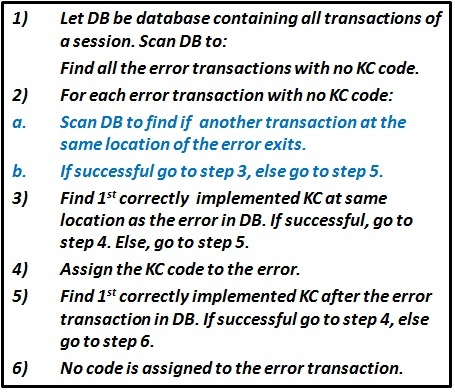
\includegraphics[scale=0.7]{LTH-1.jpg}
\caption{Algorithm for LTH-1.}
\label{LTH-1}
\end{figure}

\section{Related Work}
In \cite{Nwaigwe1}, Nwaigwe et al. have implemented various methods for error attribution in learning curve analysis in intelligent tutoring systems. They had compared the performance of two temporal and two location-temporal heuristics by evaluating the heuristics in terms of better prediction of student's changes in error-rate over time. Their analysis led to the conclusion that the location-temporal heuristic methods led to better results than the temporal heuristic methods. Our present work tries to extend their idea, where we have investigated three different location-temporal heuristics, and chose the best among them for error attribution with ANDES.

In \cite{Nwaigwe2}, Nwaigwe et al. extended their previous work on evaluating the performance of heuristic for error attribution, to a maths domain to generalize the results to different ITS domains. Their results indicate that, for tutors where the KCs can be determined by the interface location where the error occurs, the simple location heuristic was better than the simple temporal heuristic. In our paper, we also try to investigate if the use of a location-temporal heuristic with ANDES can improve student modeling.

\section{Method}
% no \IEEEPARstart

The current version of ANDES doesn't blame a knowledge component (KC) for each incorrect step (or red entry). This kind of error attribution is important to analyze student data in the form of learning curves where the error-rate is studied with each opportunity of application of a KC.

We had investigated the performance of three location-temporal (LT) heuristics: LTH-1, LTH-2 and LTH-3 for error attribution. Each of the heuristic is implemented using PHP.

\begin{figure}
\centering
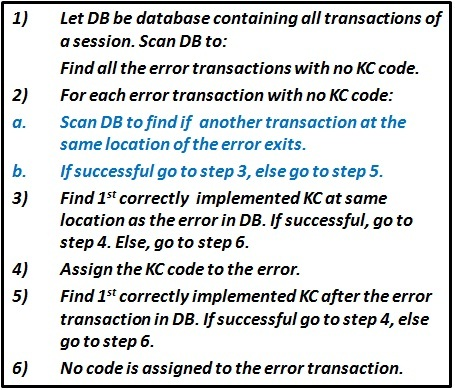
\includegraphics[scale=0.7]{LTH-2.jpg}
\caption{Algorithm for LTH-2.}
\label{LTH-2}
\end{figure}



\subsection{Location-Temporal Heuristics}
The simple temporal heuristic when used to assign a KC for an error transaction, assigns blame to the first KC the student successfully implements after the error transaction. The simple location heuristic takes into account the error location and assigns blame to the first KC, which the student successfully implements at the same location of the error. The location-temporal heuristic tries to assign KC taking into account both the location of the error as well as the next successfully implemented KC in time. We had investigated three different location-temporal heuristics for error attribution with ANDES which are described below.


The algorithm for the first location-temporal heuristic LTH-1 is shown in Fig. \ref{LTH-1}. The PHP program for the algorithm looks for error transaction from the transactions in a log file. If it is an error transaction with a missing KC, the algorithm uses the location heuristic to search the log files to find the first correctly implemented KC at the same location and assigns blame to the corresponding KC. If unsuccessful, the algorithm uses the the temporal heuristic to find the first successfully implemented KC after the error transactions and blames the corresponding KC. If the algorithm is still unable to find a KC, than no KC code is assigned to those error transactions.



The second location temporal heuristic LTH-2 looks for error transaction with no KC associated with them in the student log files. If one such transaction is found, the algorithm searches the \textit{complete problem session} to check if there is more than one entry (or transaction) at the same location as that of the error. If such an entry exists, the algorithm than narrows down to these transactions to search for a correctly implemented KC if it exits, otherwise no KC code is assigned. If no entry at the location of the error exits, the algorithm uses the temporal heuristic to assign the blame. The algorithm is shown in Fig. \ref{LTH-2}.

In third location temporal heuristic LTH-3 as shown in Fig. \ref{LTH-3}, for each error transaction with no associated KC, the algorithm checks if there is atleast one transaction, \textit{after the error transaction}, at the same location of the error. If such transactions exist, it looks for a correctly implemented KC at these locations and assigns blame to the corresponding KC if found, otherwise no KC code is assigned. If no such transaction at the location of the error exists, the algorithm uses the temporal heuristic to assign the blame.

\begin{figure}
\centering
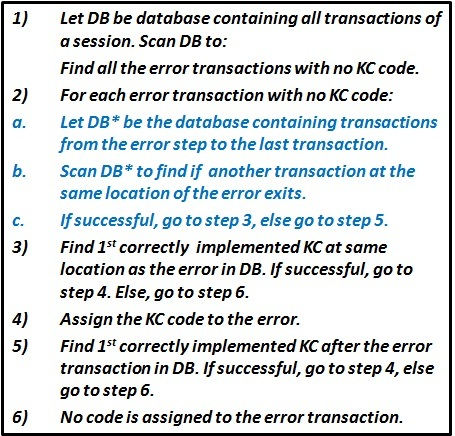
\includegraphics[scale=0.7]{LTH-3.jpg}
\caption{Algorithm for LTH-3.}
\label{LTH-3}
\end{figure}


\begin{figure*}
\centering
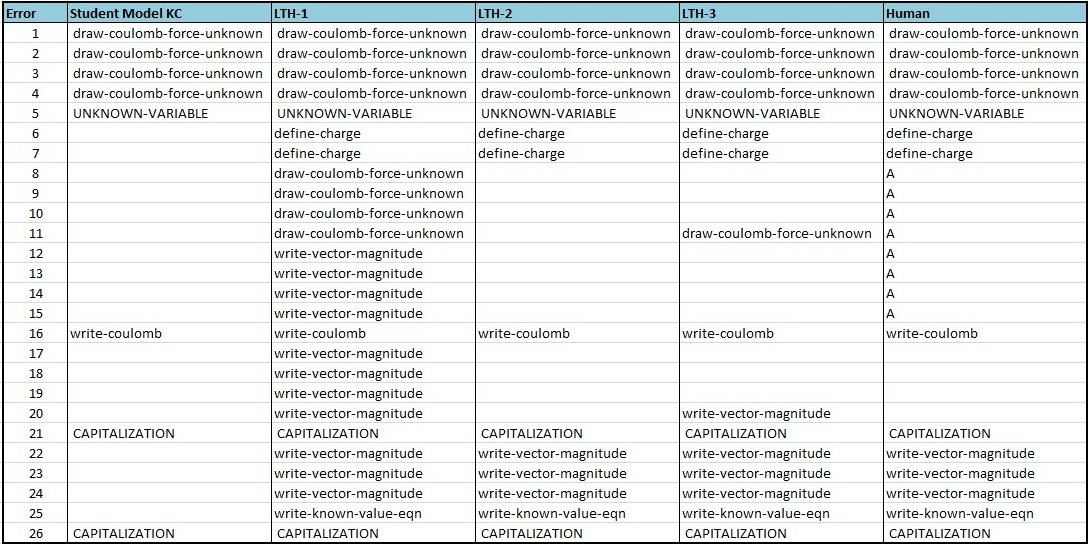
\includegraphics[scale=0.672]{Compare.jpg}
\caption{Error-attribution of KCs using different methods.}
\label{Compare}
\end{figure*}

\section{Results}

To test the accuracy of the above mentioned heuristics, they were compared against a human coder. A session consists of all the transactions of a student working on a specific problem. The errors that a student makes in a particular session were hand coded, to associate each incorrect step with a KC associated with the problem. Some errors like ``forgetting to mention units'',``not specifying the type of force'' etc. were categorized as errors occurring due to not-understanding Andes notation and coded as \textbf{A}. If the human is unable to associate a to associate any KC with a particular incorrect step, than that particular code is left black.

The same session which was hand coded, was analyzed for KC association using the heuristics LTH-1, LTH-2 and LTH-3. The codes associated by these heuristics were than compared against the human coder and the heuristic which best matches the human coder was chosen. The comparison between the codes associated by the heuristic and the codes associated by the human, was done using Fliess' generalized Kappa statistic \cite{Fliess}.

Kappa is a measure of agreement between two raters, who are independently classifying each of a sample of subjects into one of a set of mutually exclusive and exhaustive categories. Cohen's \cite{Cohen} kappa statistic is used to quantify the level of agreement between two raters while placing items, elements etc. into two or more categories. Fleiss \cite{Fliess} extended the measure to include multiple raters, denoting it the generalized kappa statistic. With regard to our problem, we are associating each error entry (or item) with a KC code (or category) and finding the Kappa statistic between the ratings by the heuristics and human coder.

The physics problems solved by students at St. Anselm college with ANDES was used for the study. As an example, Fig. \ref{Compare} shows the error-attribution of KCs using different methods for a student session with id ``sbartley\_asucoul1b1306946102432''. The student has made 26 errors, while attempting to solve a problem to find the Coulomb force on a charge Q2 by another charge Q1 using ANDES. In Fig. \ref{Compare}, \textit{student model KC} refers to the error attribution of ANDES without any heuristic, \textit{LTH-1, LTH-2 \& LTH-3} refer to the error attribution by the three heuristics and \textit{human} refers to the error attribution by human.

As a first analysis to compute the Kappa scores, all of the 26 error transactions were retained. Kappa score is calculated for each heuristic as well as the student model with respect to the human coder. The results are shown in Fig. \ref{Kappa1}, from which it is clear that implementing an error attribution algorithm is better than the student model currently used by ANDES, since the kappa score for the latter is lower than that of any heuristic. Compared to the three heuristics, LTH-2 provides better kappa score which matches the human coder.

Further analysis was done by removing the transactions which were coded as ``\textbf{A}'' by the human coder, since these errors are due to a misunderstanding of andes notation and not related to physics. The Kappa scores are shown in Fig. \ref{Kappa2}. It can be seen that the heuristic LTH-2 has better kappa score than LTH-1 and LTH-3. Also the kappa score for LTH-2 is 1, which signifies that it exactly matches the error attribution by the human coder.

\begin{figure}
  \centering
    \subfloat[Kappa scores with all the transactions retained]{\label{Kappa1}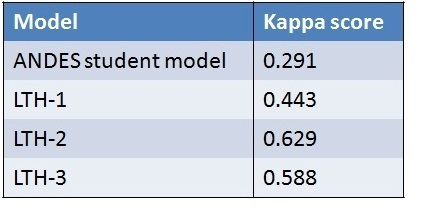
\includegraphics[scale=0.4]{Kappa1.jpg}}
    \subfloat[Kappa scores with transactions hand-coded as \textbf{A} removed]{\label{Kappa2}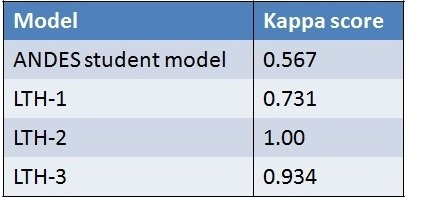
\includegraphics[scale=0.4]{Kappa2.jpg}}
   \caption{Kappa scores to access rater agrement between heuristics and human.}
    \label{Kappa}
\end{figure}

Even though heuristic LTH-1 codes more transactions than other heuristics, it doesn't perform as good as LTH-2. This is due to the fact that this heuristic assigns a code to an error transaction even though the location heuristic fails. This leads to a lot of errors being coded differently compared to that of a human, since the first correctly implemented KC code is assigned to a error transaction irrespective of the location.

LTH-2 performs better than other heuristics because it avoids assigning KC to an error transaction, if location heuristic is unable to find the KC code when there are more than one transactions at the same location as the error. This is intuitive because, if a student is working on a subtask of a problem (e.g. weight-law) and ANDES turns that entry red, and if this keeps happening many times, than student generally deletes that entry and switches to working on another subtask of the problem (e.g. define-acceleration) and returns to the original subtask later. However, this might not be possible in cases where the subtasks need to be done in a particular order like mass has to be defined before writing the weight law.

From Fig. \ref{Kappa}, it can be seen that the performance of LTH-3 is comparable to LTH-2. LTH-3 is an algorithm with performance intermediate between LTH-1 and LTH-2, as it avoids unnecessary assignment of KC codes like LTH-1 and also can handle the dependency between the subtasks better than LTH-2. We have used LTH-2 for further analysis as it performs better than the other heuristics.

\begin{table}
\caption{Kappa scores for 9 sessions to compare heuristic LTH-2 and human}
\centering
\label{Best}
\begin{tabular}{|c|c|}

\hline
{\it {\bf Session ID }} & Kappa \\
\hline
      cdupuis\_asukt3a1307547745030  &       0.649   \\

      sbartley\_asuint1b1310567135411  &        0.855 \\

      sbartley\_asus7b1306347758733 &       0.82  \\

     sbartley\_asus11a1306456523510 &      0.782  \\

    lfortin\_asus11a1306426242752 &      0.392 \\

    mconway\_asudt1a1307635165308 &    0.385 \\

    mconway\_asukt12a1308065944163&    0.797 \\

     lfortin\_asucoul2a1306857625316 &   0.775 \\

sbartley\_asucoul1b1306946102432  &       0.629   \\
\hline
\end{tabular}
\end{table}

%\begin{figure}
%\centering
%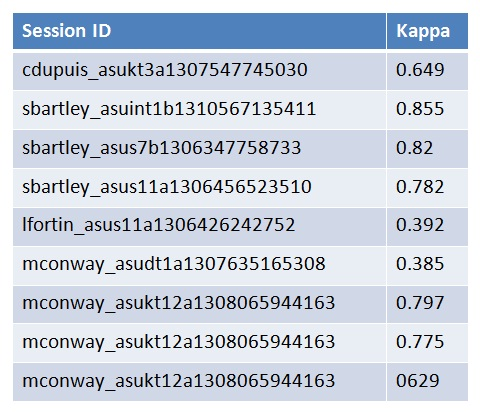
\includegraphics[scale=0.5]{Best.jpg}
%\caption{Kappa scores for 9 sessions to compare heuristic LTH-2 and human.}
%\label{Best}
%\end{figure}

A validation study was conducted to analyze the performance of the algorithm LTH-2 using the kappa statistic. The KC codes assigned by the heuristic were compared with those coded by the human. For this study, 9 physics problems solved by the students of St.Anselm colleger were used. All the error transactions with no associated KC code were used for analysis. The average kappa for the 9 sessions was found to be 0.676, which indicates a substantial agreement between the ratings of the heuristic LTH-2 and human. The kappa scores for all the 9 sessions are shown in Table \ref{Best}.



\section{Conclusion}

The current version of ANDES associates only a few error steps with knowledge components to attribute the blame. However, it is required to have more such associations to aid in analysis like student learning curves etc. In this paper we have investigated the performance of three different location-temporal heuristics for error attribution.Statistical analysis like kappa statistic was used to chose the best among the three heuristics. The best heuristic was chosen taken into account that the error attribution would match the highest to a human coder. Also, we have aimed to minimize associating irrelevant KCs to error steps which would lead to low statistic. The heuristic was implemented with ANDES to improve the usability of the log files for further analysis using tools such as Pittsburg Science of Learning Center's `DataShop' (see http://learnlab.org).

% use section* for acknowledgement
\section*{Acknowledgment}


\begin{thebibliography}{1}

\bibitem{Nwaigwe1}
Nwaigwe, Adaeze and Koedinger, Kenneth R. and Vanlehn, Kurt and Hausmann, Robert and Weinstein, Anders, \emph{Exploring Alternative Methods for Error Attribution in Learning Curves Analysis in Intelligent Tutoring Systems}.\hskip 1em plus
  0.5em minus 0.4em\relax pages 246-253, Proceedings of the 2007 conference on Artificial Intelligence in Education: Building Technology Rich Learning Contexts That Work, IOS Press, Amsterdam, The Netherlands, 2007.

\bibitem{Nwaigwe2}
Nwaigwe, Adaeze and Koedinger, Kenneth R., \emph{The Simple Location Heuristic is Better at Predicting Students' Changes in Error Rate Over Time Compared to the Simple Temporal Heuristic}.\hskip 1em plus
  0.5em minus 0.4em\relax pages 71-80, EDM 2011.

  \bibitem{Cohen}
Cohen, Jacob, \emph{A Coefficient of Agreement for Nominal Scale}.\hskip 1em plus
  0.5em minus 0.4em\relax pages 37-46, volume 20, Educational and Psychological Measurement, 1960.

 \bibitem{Fliess}
Fleiss, J.L., \emph{Measuring nominal scale agreement among many raters}.\hskip 1em plus
  0.5em minus 0.4em\relax pages 378-382, volume 76, Psychological Bulletin, 1971.


\end{thebibliography}






% that's all folks
\end{document}


